% Options for packages loaded elsewhere
\PassOptionsToPackage{unicode}{hyperref}
\PassOptionsToPackage{hyphens}{url}
\PassOptionsToPackage{dvipsnames,svgnames,x11names}{xcolor}
%
\documentclass[
  sn-nature,
]{sn-jnl}

\usepackage{amsmath,amssymb}
\usepackage{iftex}
\ifPDFTeX
  \usepackage[T1]{fontenc}
  \usepackage[utf8]{inputenc}
  \usepackage{textcomp} % provide euro and other symbols
\else % if luatex or xetex
  \usepackage{unicode-math}
  \defaultfontfeatures{Scale=MatchLowercase}
  \defaultfontfeatures[\rmfamily]{Ligatures=TeX,Scale=1}
\fi
\usepackage{lmodern}
\ifPDFTeX\else  
    % xetex/luatex font selection
\fi
% Use upquote if available, for straight quotes in verbatim environments
\IfFileExists{upquote.sty}{\usepackage{upquote}}{}
\IfFileExists{microtype.sty}{% use microtype if available
  \usepackage[]{microtype}
  \UseMicrotypeSet[protrusion]{basicmath} % disable protrusion for tt fonts
}{}
\makeatletter
\@ifundefined{KOMAClassName}{% if non-KOMA class
  \IfFileExists{parskip.sty}{%
    \usepackage{parskip}
  }{% else
    \setlength{\parindent}{0pt}
    \setlength{\parskip}{6pt plus 2pt minus 1pt}}
}{% if KOMA class
  \KOMAoptions{parskip=half}}
\makeatother
\usepackage{xcolor}
\setlength{\emergencystretch}{3em} % prevent overfull lines
\setcounter{secnumdepth}{5}
% Make \paragraph and \subparagraph free-standing
\ifx\paragraph\undefined\else
  \let\oldparagraph\paragraph
  \renewcommand{\paragraph}[1]{\oldparagraph{#1}\mbox{}}
\fi
\ifx\subparagraph\undefined\else
  \let\oldsubparagraph\subparagraph
  \renewcommand{\subparagraph}[1]{\oldsubparagraph{#1}\mbox{}}
\fi

\usepackage{color}
\usepackage{fancyvrb}
\newcommand{\VerbBar}{|}
\newcommand{\VERB}{\Verb[commandchars=\\\{\}]}
\DefineVerbatimEnvironment{Highlighting}{Verbatim}{commandchars=\\\{\}}
% Add ',fontsize=\small' for more characters per line
\usepackage{framed}
\definecolor{shadecolor}{RGB}{241,243,245}
\newenvironment{Shaded}{\begin{snugshade}}{\end{snugshade}}
\newcommand{\AlertTok}[1]{\textcolor[rgb]{0.68,0.00,0.00}{#1}}
\newcommand{\AnnotationTok}[1]{\textcolor[rgb]{0.37,0.37,0.37}{#1}}
\newcommand{\AttributeTok}[1]{\textcolor[rgb]{0.40,0.45,0.13}{#1}}
\newcommand{\BaseNTok}[1]{\textcolor[rgb]{0.68,0.00,0.00}{#1}}
\newcommand{\BuiltInTok}[1]{\textcolor[rgb]{0.00,0.23,0.31}{#1}}
\newcommand{\CharTok}[1]{\textcolor[rgb]{0.13,0.47,0.30}{#1}}
\newcommand{\CommentTok}[1]{\textcolor[rgb]{0.37,0.37,0.37}{#1}}
\newcommand{\CommentVarTok}[1]{\textcolor[rgb]{0.37,0.37,0.37}{\textit{#1}}}
\newcommand{\ConstantTok}[1]{\textcolor[rgb]{0.56,0.35,0.01}{#1}}
\newcommand{\ControlFlowTok}[1]{\textcolor[rgb]{0.00,0.23,0.31}{#1}}
\newcommand{\DataTypeTok}[1]{\textcolor[rgb]{0.68,0.00,0.00}{#1}}
\newcommand{\DecValTok}[1]{\textcolor[rgb]{0.68,0.00,0.00}{#1}}
\newcommand{\DocumentationTok}[1]{\textcolor[rgb]{0.37,0.37,0.37}{\textit{#1}}}
\newcommand{\ErrorTok}[1]{\textcolor[rgb]{0.68,0.00,0.00}{#1}}
\newcommand{\ExtensionTok}[1]{\textcolor[rgb]{0.00,0.23,0.31}{#1}}
\newcommand{\FloatTok}[1]{\textcolor[rgb]{0.68,0.00,0.00}{#1}}
\newcommand{\FunctionTok}[1]{\textcolor[rgb]{0.28,0.35,0.67}{#1}}
\newcommand{\ImportTok}[1]{\textcolor[rgb]{0.00,0.46,0.62}{#1}}
\newcommand{\InformationTok}[1]{\textcolor[rgb]{0.37,0.37,0.37}{#1}}
\newcommand{\KeywordTok}[1]{\textcolor[rgb]{0.00,0.23,0.31}{#1}}
\newcommand{\NormalTok}[1]{\textcolor[rgb]{0.00,0.23,0.31}{#1}}
\newcommand{\OperatorTok}[1]{\textcolor[rgb]{0.37,0.37,0.37}{#1}}
\newcommand{\OtherTok}[1]{\textcolor[rgb]{0.00,0.23,0.31}{#1}}
\newcommand{\PreprocessorTok}[1]{\textcolor[rgb]{0.68,0.00,0.00}{#1}}
\newcommand{\RegionMarkerTok}[1]{\textcolor[rgb]{0.00,0.23,0.31}{#1}}
\newcommand{\SpecialCharTok}[1]{\textcolor[rgb]{0.37,0.37,0.37}{#1}}
\newcommand{\SpecialStringTok}[1]{\textcolor[rgb]{0.13,0.47,0.30}{#1}}
\newcommand{\StringTok}[1]{\textcolor[rgb]{0.13,0.47,0.30}{#1}}
\newcommand{\VariableTok}[1]{\textcolor[rgb]{0.07,0.07,0.07}{#1}}
\newcommand{\VerbatimStringTok}[1]{\textcolor[rgb]{0.13,0.47,0.30}{#1}}
\newcommand{\WarningTok}[1]{\textcolor[rgb]{0.37,0.37,0.37}{\textit{#1}}}

\providecommand{\tightlist}{%
  \setlength{\itemsep}{0pt}\setlength{\parskip}{0pt}}\usepackage{longtable,booktabs,array}
\usepackage{calc} % for calculating minipage widths
% Correct order of tables after \paragraph or \subparagraph
\usepackage{etoolbox}
\makeatletter
\patchcmd\longtable{\par}{\if@noskipsec\mbox{}\fi\par}{}{}
\makeatother
% Allow footnotes in longtable head/foot
\IfFileExists{footnotehyper.sty}{\usepackage{footnotehyper}}{\usepackage{footnote}}
\makesavenoteenv{longtable}
\usepackage{graphicx}
\makeatletter
\def\maxwidth{\ifdim\Gin@nat@width>\linewidth\linewidth\else\Gin@nat@width\fi}
\def\maxheight{\ifdim\Gin@nat@height>\textheight\textheight\else\Gin@nat@height\fi}
\makeatother
% Scale images if necessary, so that they will not overflow the page
% margins by default, and it is still possible to overwrite the defaults
% using explicit options in \includegraphics[width, height, ...]{}
\setkeys{Gin}{width=\maxwidth,height=\maxheight,keepaspectratio}
% Set default figure placement to htbp
\makeatletter
\def\fps@figure{htbp}
\makeatother
% definitions for citeproc citations
\NewDocumentCommand\citeproctext{}{}
\NewDocumentCommand\citeproc{mm}{%
  \begingroup\def\citeproctext{#2}\cite{#1}\endgroup}
\makeatletter
 % allow citations to break across lines
 \let\@cite@ofmt\@firstofone
 % avoid brackets around text for \cite:
 \def\@biblabel#1{}
 \def\@cite#1#2{{#1\if@tempswa , #2\fi}}
\makeatother
\newlength{\cslhangindent}
\setlength{\cslhangindent}{1.5em}
\newlength{\csllabelwidth}
\setlength{\csllabelwidth}{3em}
\newenvironment{CSLReferences}[2] % #1 hanging-indent, #2 entry-spacing
 {\begin{list}{}{%
  \setlength{\itemindent}{0pt}
  \setlength{\leftmargin}{0pt}
  \setlength{\parsep}{0pt}
  % turn on hanging indent if param 1 is 1
  \ifodd #1
   \setlength{\leftmargin}{\cslhangindent}
   \setlength{\itemindent}{-1\cslhangindent}
  \fi
  % set entry spacing
  \setlength{\itemsep}{#2\baselineskip}}}
 {\end{list}}
\usepackage{calc}
\newcommand{\CSLBlock}[1]{\hfill\break\parbox[t]{\linewidth}{\strut\ignorespaces#1\strut}}
\newcommand{\CSLLeftMargin}[1]{\parbox[t]{\csllabelwidth}{\strut#1\strut}}
\newcommand{\CSLRightInline}[1]{\parbox[t]{\linewidth - \csllabelwidth}{\strut#1\strut}}
\newcommand{\CSLIndent}[1]{\hspace{\cslhangindent}#1}

%%%% Standard Packages

\usepackage{graphicx}%
\usepackage{multirow}%
\usepackage{amsmath,amssymb,amsfonts}%
\usepackage{amsthm}%
\usepackage{mathrsfs}%
\usepackage[title]{appendix}%
\usepackage{xcolor}%
\usepackage{textcomp}%
\usepackage{manyfoot}%
\usepackage{booktabs}%
\usepackage{algorithm}%
\usepackage{algorithmicx}%
\usepackage{algpseudocode}%
\usepackage{listings}%

%%%%

\raggedbottom
\usepackage{booktabs}
\usepackage{longtable}
\usepackage{array}
\usepackage{multirow}
\usepackage{wrapfig}
\usepackage{float}
\usepackage{colortbl}
\usepackage{pdflscape}
\usepackage{tabu}
\usepackage{threeparttable}
\usepackage{threeparttablex}
\usepackage[normalem]{ulem}
\usepackage{makecell}
\usepackage{xcolor}
\usepackage{tabularray}
\usepackage[normalem]{ulem}
\usepackage{graphicx}
\UseTblrLibrary{booktabs}
\UseTblrLibrary{siunitx}
\NewTableCommand{\tinytableDefineColor}[3]{\definecolor{#1}{#2}{#3}}
\newcommand{\tinytableTabularrayUnderline}[1]{\underline{#1}}
\newcommand{\tinytableTabularrayStrikeout}[1]{\sout{#1}}
\usepackage{multicol}
\usepackage{xcolor}
\makeatletter
\@ifpackageloaded{caption}{}{\usepackage{caption}}
\AtBeginDocument{%
\ifdefined\contentsname
  \renewcommand*\contentsname{Table of contents}
\else
  \newcommand\contentsname{Table of contents}
\fi
\ifdefined\listfigurename
  \renewcommand*\listfigurename{List of Figures}
\else
  \newcommand\listfigurename{List of Figures}
\fi
\ifdefined\listtablename
  \renewcommand*\listtablename{List of Tables}
\else
  \newcommand\listtablename{List of Tables}
\fi
\ifdefined\figurename
  \renewcommand*\figurename{Figure}
\else
  \newcommand\figurename{Figure}
\fi
\ifdefined\tablename
  \renewcommand*\tablename{Table}
\else
  \newcommand\tablename{Table}
\fi
}
\@ifpackageloaded{float}{}{\usepackage{float}}
\floatstyle{ruled}
\@ifundefined{c@chapter}{\newfloat{codelisting}{h}{lop}}{\newfloat{codelisting}{h}{lop}[chapter]}
\floatname{codelisting}{Listing}
\newcommand*\listoflistings{\listof{codelisting}{List of Listings}}
\makeatother
\makeatletter
\makeatother
\makeatletter
\@ifpackageloaded{caption}{}{\usepackage{caption}}
\@ifpackageloaded{subcaption}{}{\usepackage{subcaption}}
\makeatother
\ifLuaTeX
  \usepackage{selnolig}  % disable illegal ligatures
\fi
\usepackage{bookmark}

\IfFileExists{xurl.sty}{\usepackage{xurl}}{} % add URL line breaks if available
\urlstyle{same} % disable monospaced font for URLs
\hypersetup{
  pdftitle={Article Template},
  pdfauthor={Author One; Author Two},
  pdfkeywords={template, demo},
  colorlinks=true,
  linkcolor={blue},
  filecolor={Maroon},
  citecolor={Blue},
  urlcolor={Blue},
  pdfcreator={LaTeX via pandoc}}

\title[Article Template]{Article Template}

% author setup
\author[1,2]{\fnm{Author} \sur{One}}\equalcont{These authors contributed equally to this work.}\author*[1]{\fnm{Author} \sur{Two}}\email{corresponding@email.com}\equalcont{These authors contributed equally to this work.}
% affil setup
\affil[1]{\orgdiv{Social Sciences}, \orgname{Humboldt
University}, \orgaddress{\street{street}, \city{Berlin}, \postcode{12345}}}
\affil[2]{\orgdiv{IPI}, \orgname{WZB}, \orgaddress{\street{here}, \city{Berlin}, \postcode{12345}}}

% abstract 

\abstract{The abstract serves both as a general introduction to the
topic and as a brief, non-technical summary of the main results and
their implications. Authors are advised to check the author instructions
for the journal they are submitting to for word limits and if structural
elements like subheadings, citations, or equations are permitted.}

% keywords
\keywords{template,  demo}

\begin{document}
\maketitle

\newpage

\section{Introduction}\label{sec-intro}

This template is based on the quarto template provided by Christopher
Kenny. Note a range of different templates are available with various
options: consult https://github.com/christopherkenny/nature

Your question. why we care

Your findings and the contribution

Roadmap

\section{Motivation: Theory, Literature}\label{sec-motivation}

You can use \LaTeX natively. See Equation~\ref{eq-euclid}.

\begin{equation}\phantomsection\label{eq-euclid}{
f(x) = -\frac{1}2(1-x)^2
}\end{equation}

\newpage

\section{Results}\label{results}

Tables and Figures can be produced on the fly or imported.

\subsection{A sample figure}\label{a-sample-figure}

Here is figure produced on the fly. See Figure~\ref{fig-1}. Code is
shown but you would hide this by setting \texttt{echo:\ false}

\begin{Shaded}
\begin{Highlighting}[]
\FunctionTok{read\_rds}\NormalTok{(}\StringTok{"data/data.rds"}\NormalTok{) }\SpecialCharTok{|\textgreater{}}
  \FunctionTok{ggplot}\NormalTok{(}\FunctionTok{aes}\NormalTok{(X, Y)) }\SpecialCharTok{+} \FunctionTok{geom\_point}\NormalTok{()}
\end{Highlighting}
\end{Shaded}

\begin{figure}[H]

\centering{

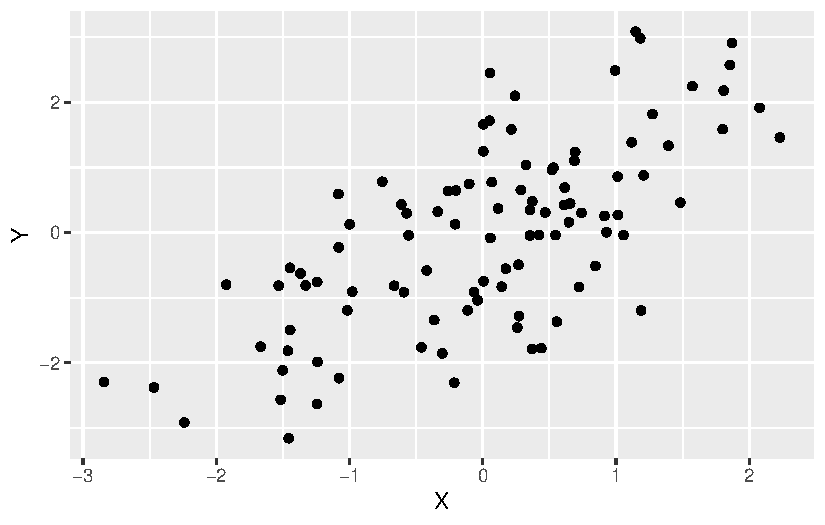
\includegraphics{my_paper_files/figure-pdf/fig-1-1.pdf}

}

\caption{\label{fig-1}sample figure}

\end{figure}%

\newpage

\subsection{A sample summary stats
table}\label{a-sample-summary-stats-table}

Produced on the fly. See Table~\ref{tbl-simple}.

\begin{Shaded}
\begin{Highlighting}[]
\FunctionTok{read\_rds}\NormalTok{(}\StringTok{"data/data.rds"}\NormalTok{) }\SpecialCharTok{|\textgreater{}}
  \FunctionTok{summarize}\NormalTok{(}\StringTok{\textasciigrave{}}\AttributeTok{mean Y}\StringTok{\textasciigrave{}} \OtherTok{=} \FunctionTok{mean}\NormalTok{(Y), }
            \StringTok{\textasciigrave{}}\AttributeTok{mean X}\StringTok{\textasciigrave{}} \OtherTok{=} \FunctionTok{mean}\NormalTok{(X), }
            \AttributeTok{correlation =} \FunctionTok{cor}\NormalTok{(X, Y)) }\SpecialCharTok{|\textgreater{}}
  \FunctionTok{kable}\NormalTok{(}\AttributeTok{digits =} \DecValTok{2}\NormalTok{, }\AttributeTok{caption =} \StringTok{"A sample table"}\NormalTok{)}
\end{Highlighting}
\end{Shaded}

\begin{longtable}[]{@{}rrr@{}}

\caption{\label{tbl-simple}A sample table}

\tabularnewline

\toprule\noalign{}
mean Y & mean X & correlation \\
\midrule\noalign{}
\endhead
\bottomrule\noalign{}
\endlastfoot
-0.03 & 0.02 & 0.69 \\

\end{longtable}

\newpage

\subsection{Analysis in parallel}\label{analysis-in-parallel}

Produced on the fly.

\begin{Shaded}
\begin{Highlighting}[]
\CommentTok{\# generate a list of models}
\NormalTok{two\_models }\OtherTok{\textless{}{-}} 
  \FunctionTok{list}\NormalTok{(}
  \FunctionTok{lm\_robust}\NormalTok{(Y}\SpecialCharTok{\textasciitilde{}}\DecValTok{1}\NormalTok{, }\AttributeTok{data =} \FunctionTok{read\_rds}\NormalTok{(}\StringTok{"data/data.rds"}\NormalTok{)),}
  \FunctionTok{lm\_robust}\NormalTok{(Y}\SpecialCharTok{\textasciitilde{}}\NormalTok{X, }\AttributeTok{data =} \FunctionTok{read\_rds}\NormalTok{(}\StringTok{"data/data.rds"}\NormalTok{)))}
\end{Highlighting}
\end{Shaded}

\newpage

\subsection{Analysis output}\label{analysis-output}

Then print. Here using \texttt{modelsummary}. Lots of scope for
customization: https://modelsummary.com/articles/appearance.html

\begin{table}

\caption{\label{tbl-ols}}

\centering{

\captionsetup{labelsep=none}

\begin{Shaded}
\begin{Highlighting}[]
\CommentTok{\# print nicely}
\NormalTok{two\_models}\SpecialCharTok{|\textgreater{}}
  \FunctionTok{modelsummary}\NormalTok{(}\AttributeTok{caption =} \StringTok{": some analyses"}\NormalTok{, }\AttributeTok{note =} \StringTok{"some notes"}\NormalTok{) }
\end{Highlighting}
\end{Shaded}

\centering
\begin{talltblr}[         %% tabularray outer open
entry=none,label=none,
note{}={some notes},
]                     %% tabularray outer close
{                     %% tabularray inner open
colspec={Q[]Q[]Q[]},
column{1}={halign=l,},
column{2}={halign=c,},
column{3}={halign=c,},
hline{6}={1,2,3}{solid, 0.05em, black},
}                     %% tabularray inner close
\toprule
& (1) & (2) \\ \midrule %% TinyTableHeader
(Intercept) & \num{-0.033}  & \num{-0.050}  \\
& (\num{0.143}) & (\num{0.104}) \\
X           &                & \num{0.941}   \\
&                & (\num{0.083}) \\
Num.Obs.    & \num{100}     & \num{100}     \\
R2          & \num{0.000}   & \num{0.478}   \\
R2 Adj.     & \num{0.000}   & \num{0.473}   \\
AIC         &                & \num{295.7}   \\
BIC         &                & \num{303.6}   \\
RMSE        &                & \num{1.03}    \\
\bottomrule
\end{talltblr}

}

\end{table}%

\newpage

\section{Referencing and cross
referencing}\label{referencing-and-cross-referencing}

\subsection{Cross Referencing}\label{cross-referencing}

\begin{itemize}
\tightlist
\item
  To reference a figure with example label ``plot'', use
  e.g.~\texttt{@fig-plot}. Figure~\ref{fig-1}
\item
  Analogously, to reference a table with example label ``data'', use
  e.g.~\texttt{@tbl-data}. Table~\ref{tbl-simple}.
\item
  To reference a section, such as the Introduction
  (Section~\ref{sec-intro}), use e.g.~\texttt{@sec-intro}.
\item
  To reference an equation, same (Equation~\ref{eq-euclid}), use
  e.g.~\texttt{@eq-euclid}.
\end{itemize}

For complete information on cross referencing with Quarto, see
\url{https://quarto.org/docs/authoring/cross-references.html}.

\subsection{Citations}\label{citations}

\begin{itemize}
\tightlist
\item
  For a citation in parentheses use \texttt{{[}@putnam2000bowling{]}}
  and for a text citation: \texttt{@putnam2000bowling}.
\item
  These render as (Putnam 2000) and Putnam (2000)
\end{itemize}

Multiple citations can be given as
\texttt{{[}@putnam2000bowling;@blair2023research{]}}, producing (Putnam
2000; Blair et al. 2023)

\newpage

\section{References}\label{references}

\phantomsection\label{refs}
\begin{CSLReferences}{1}{1}
\bibitem[\citeproctext]{ref-blair2023research}
Blair G, Coppock A, Humphreys M (2023) Research design in the social
sciences: Declaration, diagnosis, and redesign. Princeton University
Press

\bibitem[\citeproctext]{ref-putnam2000bowling}
Putnam RD (2000) Bowling alone: America's declining social capital. In:
Culture and politics. Springer, pp 223--234

\end{CSLReferences}



\end{document}
